\documentclass{uebungszettel}
\geometry{bmargin=2.8cm,tmargin=1.5cm}

\usepackage{framed}
\usepackage{textcomp}
\usepackage{dashrule}

\begin{document}

\pagestyle{plain}
\setlength{\aufgabenskip}{1.5em}

\begin{picture}(0,0)
 \put(0,-4.5){  \vbox{  Mathesch\"ulerzirkel\\
   Universit\"at Augsburg\\
%  Schuljahr 2015/2016\\
  Tag der Mathematik 2016 \\\ \\
  Hast du Lust auf spannende Mathematik abseits des Schulunterrichts? \\
  Dann geh auf \url{http://www.math.uni-augsburg.de/schueler/mathezirkel/} \\
  und informiere dich über den Matheschülerzirkel Augsburg. \\\ \\
  Da gibt es zweiwöchentliche Seminare auf dem Campus in kleinen Gruppen und \\
  Korrespondenz per Post. Außerdem ein großes Mathecamp in den Sommerferien. \\\ \\
  Man kann jederzeit reinschnuppern!}}
 \put(14,-2){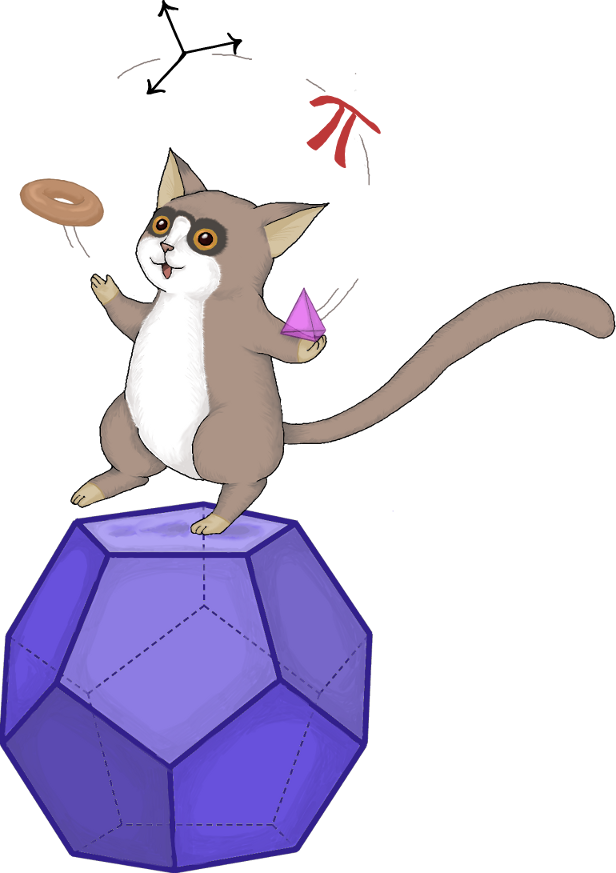
\includegraphics[scale=0.10]{Bilder/cover} }
\end{picture} \vspace*{5.7cm}
  \begin{center}\Large \textbf{Binärzahlen}
  \end{center}
  \vspace{\titleskip}

\thispagestyle{plain}

Um Zahlen aufzuschreiben benutzen wir heutzutage das 10er-System: Zum Beispiel steht die Zeichenfolge \glqq 113\grqq \ für die Zahl
\[\begin{array}{llll}
& 1 \cdot 100 & + \quad 1 \cdot 10 & + \quad 3 \cdot 1\\
= & 1 \cdot 10^2 & + \quad 1 \cdot 10^1 & + \quad 3 \cdot 10^0
\end{array}\]
und die Zeichenfolge \glqq 2079\grqq \ für
\[\begin{array}{lllll}
& 2 \cdot 1000 & + \quad 0 \cdot 100 & + \quad 7 \cdot 10 & + \quad 9 \cdot 1\\
= & 2 \cdot 10^3 & + \quad 0 \cdot 10^2 & + \quad 7 \cdot 10^1 & + \quad 9 \cdot 10^0.
\end{array}\]

Man kann aber auch andere Zahlen anstatt der 10 benutzen und erhält auf diese Weise andere Zeichenfolgen für dieselbe Zahl. Im 2er-System würde man z.\,B. die Zahl 113 so notieren: \glqq 1110001\grqq . Das folgt aus folgender Rechnung:
\[\begin{array}{llllllll}
113 & = \quad 1 \cdot 64 & + \quad 1 \cdot 32 & + \quad 1 \cdot 16 & + \quad 0 \cdot 8 & + \quad 0 \cdot 4 & + \quad 0 \cdot 2 & + \quad 1 \cdot 1\\
& = \quad 1 \cdot 2^6 & + \quad 1 \cdot 2^5 & + \quad 1 \cdot 2^4 & + \quad 0 \cdot 2^3 & + \quad 0 \cdot 2^2 & + \quad 0 \cdot 2^1 & + \quad 1 \cdot 2^0.
\end{array}\]

Um bei den verschiedenen Zeichenfolgen für ein und dieselbe Zahl nicht durcheinander zu kommen, wird die Zeichenfolge in eckigen Klammern geschrieben und das System, in dem diese zu lesen ist, unten an die rechte Klammer gesetzt. Es gilt also z.\,B. $[113]_{10} = [1110001]_2$.

\begin{aufgabe}{Computer benutzen das Binärsystem}
Das 2er-System wird auch \emph{Binärsystem} oder auch \emph{Dualsystem} genannt.

Computer rechnen ausschließlich darin. Wieso?
\end{aufgabe}

\vspace{2 cm}
\begin{aufgabe}{Bits und Bytes}
 Die kleinste Einheit im Computer zum Speichern von Daten ist ein Bit.
 Ein solches kann entweder den Wert 0 oder 1 haben.
 Die nächstgrößere Speichereinheit ist 1 Byte -- es besteht aus 8 Bits.
 Wie viele verschiedene Zahlen kann man mit einem Byte darstellen?
\end{aufgabe}




\pagebreak



\begin{aufgabe}{Umrechnen zwischen Dezimal- und Binärsystem}
Unser übliches 10er-System wird \emph{Dezimalsystem} genannt.

Rechne folgende Zahlen vom Dezimal- in das Binärsystem um:

\[\begin{array}{rr}
[3]_{10} = & \rule{13cm}{0.5px} %\quad \quad \quad \quad \quad \quad \quad \quad \quad \quad \quad \quad \quad \quad \quad \quad \quad \quad \quad \quad \quad \quad \quad \quad \quad \quad \quad \quad \quad \quad\\
\\\\\\
\left[ 7 \right]_{10} = & \rule{13cm}{0.5px}\\
\\\\
\left[ 12 \right]_{10} = & \rule{13cm}{0.5px}\\
\\\\
\left[ 25 \right]_{10} = & \rule{13cm}{0.5px}\\
\\\\
\left[ 59 \right]_{10} = & \rule{13cm}{0.5px}\\
\end{array}\]

\vspace{1 cm}
Rechne folgende Zahlen vom Binär- in das Dezimalsystem um:

\[\begin{array}{rr}
[10]_{2} = & \rule{12cm}{0.5px}%\quad \quad \quad \quad \quad \quad \quad \quad \quad \quad \quad \quad \quad \quad \quad \quad \quad \quad \quad \quad \quad \quad \quad \quad \quad \quad \quad \quad \quad \quad\\
\\\\\\
\left[ 101 \right]_{2} = & \rule{12cm}{0.5px}\\
\\\\
\left[ 110 \right]_{2} = & \rule{12cm}{0.5px}\\
\\\\
\left[ 1011 \right]_{2} = & \rule{12cm}{0.5px}\\
\\\\
\left[ 10011 \right]_{2} = & \rule{12cm}{0.5px}\\
\\\\
\left[ 101110 \right]_{2} = & \rule{12cm}{0.5px}\\
\end{array}\]
\end{aufgabe}

%\pagebreak

\begin{aufgabe}{Addition im Binärsystem}
Addiere schriftlich folgende Zahlen im Binärsystem. Beachte dabei für den Übertrag der 1, dass $[1]_2 + [1]_2 = [10]_2$ gilt.
\[\begin{array}{rrrrrrrrr}
[10]_{2} & \quad \quad \quad & \left[ 1 \right]_2 & \quad \quad \quad & \left[ 111 \right]_2 & \quad \quad \quad & \left[ 110001 \right]_2 \\
+ \quad \quad \left[ 10 \right]_{2} & & + \quad \quad \left[ 101 \right]_2 & & + \quad \quad \left[ 1011 \right]_2 & & + \quad \quad \left[ 101101 \right]_2 \\
\hrulefill & & \hrulefill & & \hrulefill & & \hrulefill\\
= \hfill & & = \hfill & & = \hfill & & = \hfill
\end{array}\]
\end{aufgabe}

\pagebreak
\Large
\begin{center}
 \textbf{Die Erklärung des Zaubertricks}
\end{center}
\normalsize

Zunächst können wir die ausgelegten Münzen viermal wie folgt zerlegen:

\begin{center}
 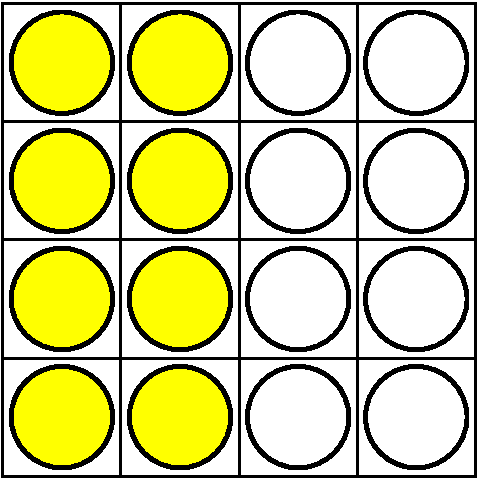
\includegraphics[scale = 0.4]{zerlegung1}\hspace*{3 mm}
 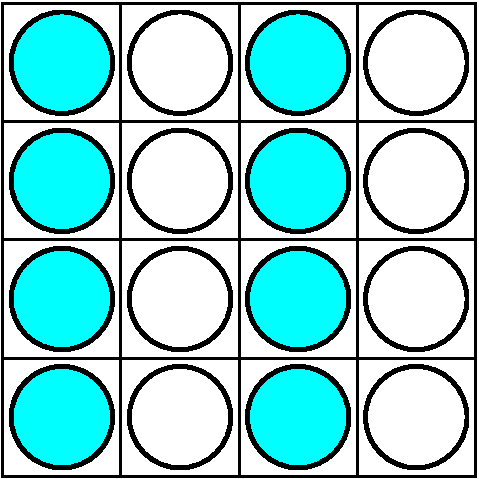
\includegraphics[scale = 0.4]{zerlegung2}\hspace*{3 mm}
 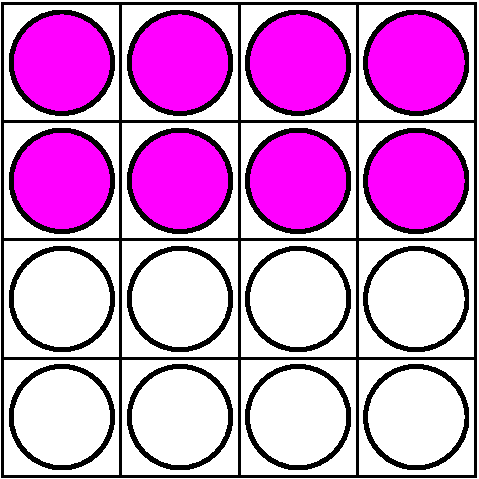
\includegraphics[scale = 0.4]{zerlegung3}\hspace*{3 mm}
 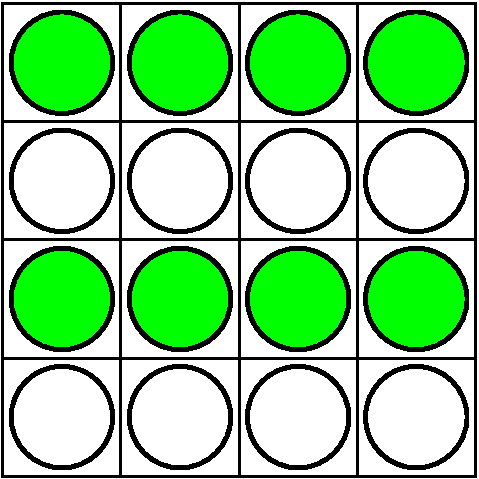
\includegraphics[scale = 0.4]{zerlegung4}
\end{center}

Entscheidend an diesen Mustern ist, dass es Münzen gibt, die in gar keiner, in genau einer, in genau zwei, in genau drei und in allen vier Zerlegungen enthalten sind.

Zuerst gehen wir jetzt darauf ein, was die Zauberin tut, wenn ein solches Münzfeld vor ihr liegt.
Wir starten mit der gelben Zerlegung.
Unter allen im Bild gelb markierten Münzen zählt die Zauberin die Anzahl Münzen, die Zahl zeigen.
Ist diese Zahl gerade, merkt (oder notiert) sie sich die Ziffer 0, ansonsten die Ziffer 1.
Dieses Vorgehen wird für die anderen drei Muster wiederholt, so dass die Zauberin nun vier Ziffern  
ermittelt hat, die jeweils 0 oder 1 sein können.

Diese vier Ziffern werden nun als Binärzahl interpretiert und 
in das Dezimalsystem umgerechnet.
%Die erste Zahl im Dezimalsystem soll der Zeile entsprechen, in der die Münze sich befindet, 
%die zweite der Spalte.

\begin{aufgabe}{Wir testen das an einem Beispiel}
 Ermittle die Dezimalzahlen im folgenden Beispiel:
 \begin{center}
 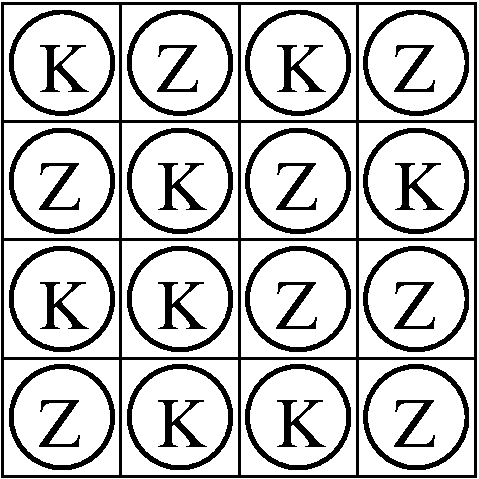
\includegraphics[scale = 0.4]{beispielbild}
\end{center}
 Man erhält stets eine Zahl zwischen 0 und 15 -- wieso?
 Daher ist es sinnvoll, die Felder von 0 bis 15 zu nummerieren. Wie man das macht, ist prinzipiell egal, solange Zauberin und Assistent sich einig sind.
 Der Einfachheit halber kann man die Felder von oben links nach unten rechts zeilenweise nummerieren.
\end{aufgabe}

%Jetzt kommt der Assistent ins Spiel, denn tatsächlich hat er die meiste Arbeit in diesem Trick.
Wenn das Publikum sich für eine Münze entschieden hat, muss die Zauberin prüfen, 
ob die Zahlen, die man bei obiger Berechnung erhält, bereits die korrekte Position dieser Münze verraten.
Wenn ja, muss sie nichts weiter machen.
Wenn nein, muss sie durch das Umlegen \emph{einer} Münze 
die korrekte Position angeben.
Dazu muss sie nur prüfen, welche Ziffern der Binärzahl noch falsch sind.
Im Anschluss dreht sie eine Münze um, die in allen Zerlegungen enthalten ist, für die eine falsche Ziffer herauskommt, 
jedoch nicht in den übrigen Zerlegungen mit bereits korrektem Ergebnis enthalten ist.
Sind beispielsweise alle vier Ziffern falsch, dreht sie einfach die Münze links oben um.

Wenn nun der Assistent den Raum betritt und das Spielfeld das erste Mal sieht, berechnet er die Position.

\begin{aufgabe}{Probiere es aus!}
 Welche Münze müssten wir im obigen Beispiel umdrehen, 
 wenn wir dem Assistenten die Position $11$ mitteilen wollen? %(Also Zeile zwei und Spalte drei!)
\end{aufgabe}

















\pagebreak

\begin{aufgabe}{Multiplikation im Binärsystem}
Multipliziert man im Dezimalsystem eine Zahl mit 10, so wird einfach eine Null an die Ziffernfolge drangehängt. Wieso ist das der Fall?

Mit welcher Zahl muss man im Binärsystem multiplizieren, damit das Ergebnis einfach durch Dranhängen einer Null an die Ziffernfolge entsteht? Durch welche Zeichenfolge wird diese Zahl im Binärsystem dargestellt?

Multipliziere schriftlich folgende Zahlen im Binärsystem:
\[\begin{array}{rrrrrrrrr}
[101]_{2} \cdot [11]_2 & \quad \quad \quad \quad \quad \quad & \left[ 11 \right]_2 \cdot [110]_2 & \quad \quad \quad \quad \quad \quad & \left[ 1010 \right]_2 \cdot [1101]_2\\
\hrulefill & & \hrulefill & & \hrulefill\\
\end{array}\]
\vspace{2cm}
\end{aufgabe}



\begin{aufgabe}{Kommazahlen}
 Natürlich kann man auch Kommazahlen mit dem Binärsystem (oder anderen Zahlensystemen) darstellen:
 \begin{itemize}
 \item [a)] $\left[ 1{,}01 \right]_{2} $
 \item [b)] $\left[ 1{,}101 \right]_{2} $
 \end{itemize} 
Überlege dir anhand der vorigen Aufgaben wie man diese Zahlen zurück in die Dezimaldarstellung bringt.

\emph{Tipp:} Im gewohnten 10er-System geben die Ziffern nach dem Komma die Zehntel, Hundertsel, Tausendstel und so weiter an. Im Binärsystem sind
es dagegen die Halben, Viertel, Achtel, Sechszehntel und so weiter.
\end{aufgabe}

\vspace{5 cm}
\begin{aufgabe}{Mit den Fingern zählen}
Wie kann man mit den Fingern von 0 bis 1023 zählen?
\end{aufgabe}

\pagebreak
\vspace{-2 mm}
\begin{aufgabe}{Das Sexagesimalsystem}
Die Babylonier verwendeten ab ungefähr 2000 v. Chr. das 60er-System (Sexagesimalsystem). In ihrer Keilschrift sah das dann so aus:
\begin{center}
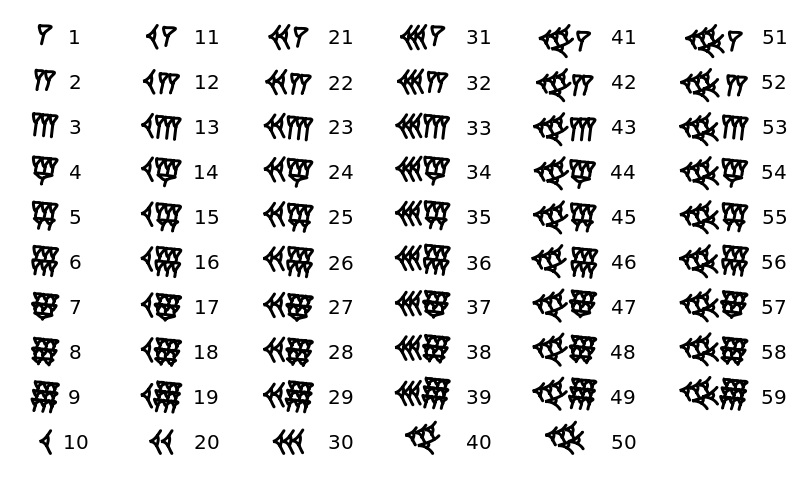
\includegraphics[scale=0.5]{Bilder/60er-System.png} 
\end{center}

Die Zahlen ab 60 wurden dann mit dem üblichen Stellenwertsystem geschrieben. Da sie jedoch zu Beginn noch kein Zeichen für die Null kannten, gab es manchmal Missverständnisse bei der Lesung.

Das Sexagesimalsystem hat sich in bestimmten Bereichen bis heute erhalten. Zum Beispiel hat eine Stunde 60 Minuten und eine Minute hat 60 Sekunden.

In manchen Teilen der Türkei, des Iraks, in Indien und in Indochina wird auch heute noch mit zwei Händen bis 60 gezählt (anstatt wie bei uns bis 10). Dazu 
wird mit einer Hand ein Dutzend (= 12) abgezählt und mit der anderen \glqq merkt\grqq \ man sich wie viele Dutzend man schon gezählt hat. Versuche 
herauszufinden, wie das genau funktioniert!\\

Schreibe 133 in Keilschrift: $\rule{10.5cm}{0.5px}$
\end{aufgabe}



%\pagebreak

\begin{aufgabe}{ASCII-Code}
 Der ASCII-Code ist eine Zeichenkodierung und wird oft mithilfe des Hexadezimalsystems dargestellt.
 Hier ist die entsprechende Basis nicht 2 wie beim Binärcode, sondern 16. Also muss man sechzehn verschiedene Ziffern verwenden. Daher zweckentfremdet man
 die ersten sechs Buchstaben als weitere Ziffern.
 
\begin{tabular}{ c c c c c c c c c c c c c c c c c c c}
    0 & 1 & 2 & 3 & 4 & 5 & 6 & 7 & 8 & 9 & 10 & 11 & 12 & 13 & 14 & 15 & 16 & 17 & \ldots \\
    0 & 1 & 2 & 3 & 4 & 5 & 6 & 7 & 8 & 9 & A  & B  & C  & D  & E  & F & 10 & 11 & \ldots
 \end{tabular}

Für zwei Hexziffern benötigt man daher ein Byte -- wieso?
Kannst du den folgenden Code entziffern?
Du musst dazu die Hexziffern in Dezimalzahlen umrechnen und in einer ASCII-Tabelle die jeweiligen Zeichen nachsehen.
Eine solche Tabelle findest du im Internet (such einfach nach \emph{ASCII-Tabelle}).
\begin{center}
48 \ 61 \ 6C \ 6C \ 6F \ 20 \ 57 \ 65 \ 6C \ 74 \ 21
 \end{center}
\end{aufgabe}

\pagebreak
\begin{aufgabe}{Binärcodes}
 Tom wurde versehentlich im Kaufhaus eingeschlossen.
 Er möchte aber unbedingt mit seinen Weihnachtseinkäufen nach Hause.
 Er hat schon gerufen, aber niemand hört ihn. Jedoch brennt im Gebäude gegenüber noch Licht.
 Tom versucht es mithilfe der Weihnachtsbeleuchtung mit einem Binärcode -- kannst du ihn entschlüsseln?
  \begin{center}
\includegraphics[scale=0.6]{Bilder/zirkel-bin1.png} 
\end{center}
  \begin{center}
\includegraphics[scale=0.6]{Bilder/zirkel-bin2.png} 
\end{center}
\end{aufgabe}

%\pagebreak
\begin{aufgabe}{Ein weiterer Zaubertrick}
 Für den Zaubertrick werden 25 Karten beliebig im Quadrat ausgelegt, wobei die Karten auf der einen Seite weiß sind und auf der anderen schwarz.
 Welche Seite sichtbar sein soll, darf das Publikum entscheiden.
 Nun ergänzt die Zauberin -- um es schwerer zu machen -- eine sechste Reihe rechts und unten.
 Danach verbindet sie sich die Augen.
 Das Publikum darf jetzt eine Karte umdrehen -- egal welche.
 Anschließend sagt die Zauberin, welche Karte umgedreht wurde!
\begin{itemize}
 \item [a)] Wie macht sie das?
 \item [b)] Was passiert, wenn zwei Karten umgedreht werden? 
 \item [c)] Muss man mit 25 Karten starten?
 \item [d)] Wie kann man dieses Wissen für Datenübertragungen nutzen? 
\end{itemize}
\end{aufgabe}




\pagebreak

\end{document}
